\documentclass[12pt,a4paper,oneside]{report}
\usepackage[utf8]{inputenc}
\usepackage[english,russian]{babel}
\usepackage{amsmath}
\usepackage{amssymb}
\usepackage{geometry}
\usepackage{sverb}
\usepackage{graphicx}
\usepackage{pdfpages}
\usepackage{hyperref} 
\usepackage{url}
\usepackage{titlesec, blindtext, color}
\usepackage{listings}
\usepackage{pgfplots}
\pgfplotsset{compat=newest}
\graphicspath{{../}}
\DeclareGraphicsExtensions{.pdf,.png,.jpg}
\usepackage{tabularx}
\usepackage{subcaption}
\usepackage{colortbl}
\usepackage{multirow}
\usepackage{longtable}
\usepackage{enumitem}
\usepackage{algorithm}
\usepackage{tikz}
\usepackage[noend]{algpseudocode}
\usepackage{float}
\definecolor{gray75}{gray}{0.75}
\definecolor{Blue}{HTML}{5D8AA8}
\newcommand{\hsp}{\hspace{20pt}}

\newcommand{\RomanNumeralCaps}[1]
{\MakeUppercase{\romannumeral #1}}



% Для листинга кода:
\lstset{ %
	language=c,                 % выбор языка для подсветки (здесь это С)
	basicstyle=\small\sffamily, % размер и начертание шрифта для подсветки кода             % где поставить нумерацию строк (слева\справа)
	numberstyle=\tiny,           % размер шрифта для номеров строк
	stepnumber=1, 
	keywordstyle=\color{blue},% размер шага между двумя номерами строк
	numbersep=5pt,                % как далеко отстоят номера строк от подсвечиваемого кода
	showspaces=false,            % показывать или нет пробелы специальными отступами
	showstringspaces=false,      % показывать или нет пробелы в строках
	showtabs=false,             % показывать или нет табуляцию в строках
	frame=single,              % рисовать рамку вокруг кода
	tabsize=2,                 % размер табуляции по умолчанию равен 2 пробелам
	captionpos=t,              % позиция заголовка вверху [t] или внизу [b] 
	breaklines=true,           % автоматически переносить строки (да\нет)
	breakatwhitespace=false, % переносить строки только если есть пробел
	escapeinside={\#*}{*)}  % Стиль литералов
}


\titleformat{\chapter}[hang]{\Huge\bfseries}{\thechapter.\textcolor{gray75}\hsp}{0pt}{\Huge\bfseries}
\newcommand{\specchapter}[1]{\chapter*{#1}\addcontentsline{toc}{chapter}{#1}}
\newcommand{\specsection}[1]{\section*{#1}\addcontentsline{toc}{section}{#1}}
\newcommand{\specsubsection}[1]{\subsection*{#1}\addcontentsline{toc}{subsection}{#1}}

% геометрия
\geometry{pdftex, left = 3cm, right = 1cm, top = 2cm, bottom = 2cm}


\setcounter{tocdepth}{4} % фикс переноса 
\righthyphenmin = 2
\tolerance = 2048


\thispagestyle{empty}



\begin{document}


\thispagestyle{empty}

\thispagestyle{empty}
\noindent \begin{minipage}{0.15\textwidth}
	
\includegraphics[width=\linewidth]{b_logo}
\end{minipage}
\noindent\begin{minipage}{0.9\textwidth}\centering
	\textbf{Министерство науки и высшего образования Российской Федерации}\\
	\textbf{Федеральное государственное бюджетное образовательное учреждение высшего образования}\\
	\textbf{«Московский государственный технический университет имени Н.Э.~Баумана}\\
	\textbf{(национальный исследовательский университет)»}\\
	\textbf{(МГТУ им. Н.Э.~Баумана)}
\end{minipage}
\noindent\rule{18cm}{3pt}
\newline\newline
\noindent ФАКУЛЬТЕТ $\underline{\textbf{«ИНФОРМАТИКА И СИСТЕМЫ УПРАВЛЕНИЯ»}}$ \newline\newline
\noindent КАФЕДРА $\underline{\textbf{«ПРОГРАММНОЕ ОБЕСПЕЧЕНИЕ ЭВМ И ИНФОРМАЦИОННЫЕ}}$\newline\newline $\underline{\textbf{ТЕХНОЛОГИИ»(ИУ7)}}$\newline\newline
\noindent НАПРАВЛЕНИЕ ПОДГОТОВКИ $\underline{\textbf{09.03.04 ПРОГРАММНАЯ ИНЖЕНЕРИЯ}}$\newline\newline\newline\newline\newline\newline\newline
\begin{center}
    \begin{flushright}
    \Large\textbf{ОТЧЕТ}\newline
	\Large\textbf{по лабораторной работе № 1}\newline
	\end{flushright}
\end{center}
\noindent\textbf{Название:} $\underline{\text{Распределение случайных величин}}$\newline\newline
\noindent\textbf{Дисциплина:} $\underline{\text{Моделирование}}$\newline\newline\newline\newline\newline\newline\newline\newline
\begin{tabular}{lcp{5em}lp{2em}l}
	\noindent\textbf{Студент} &  $\underline{\text{ИУ7-71Б~~}}$ &             &\hspace{1cm} & & $\underline{\text{В.С.Плотников}}$ \\\cline{4-3}
	 & (Группа) & &(Подпись,дата)  & & (И.О.Фамилия) \\
	 & & & & &\\
	\noindent\textbf{Преподаватель} &  & &\hspace{1cm} & &$\underline{\text{И.В.Рудаков ~~~~}}$ \\\cline{4-3} 
	 &  & & (Подпись,дата)  & &(И.О.Фамилия) \\
    \end{tabular}
\begin{center}
	\vfill
	Москва, \the\year
\end{center}
\clearpage

% \section*{Нормальное распределение}
% \quad Нормальное распределение - распределение вероятностей, которое в одномерном случае задаётся функцией плотности вероятности, совпадающей с функцией Гаусса:
% \begin{equation}
%     f(x) = \frac{1}{\sigma \sqrt{2 \pi}} e^\frac{-(x-\mu)^2}{2\sigma^2}
% \end{equation}
% где параметр $\mu$ — математическое ожидание (среднее значение), медиана и мода распределения, а параметр $\sigma$ - среднеквадратическое отклонение ($\sigma^2$ - дисперсия) распределения.

% Функция распределения:
% \begin{equation}
%     F(x) = \frac{1}{\sigma \sqrt{2 \pi}} \int_{-\infty}^x e^\frac{-(x-\mu)^2}{2\sigma^2}dx
% \end{equation}

% Обозначают нормальное распределение $X \sim N(\mu, \sigma^2)$.

% Стандартным нормальным распределением называется нормальное распределение с математическим ожиданием $\mu$ = 0 и стандартным отклонением $\sigma$ = 1.

% Математическое ожидание $\mu$ характеризует положение «центра тяжести» вероятностной массы нормального распределения. Получается, что график плотности распределения случайной величины, имеющей нормальное распределение, симметричен относительно x = $\mu$.  Дисперсия $\sigma$ характеризует разброс значений случайной величины относительно «центра тяжести». 
\section*{Задание}
\quad Реализовать программу для построения графиков функции распределения и
функции плотности распределения для следующих распределений:
\begin{itemize}
    \item распределение Пуассона;
    \item равномерное распределение.
\end{itemize}

\section*{Распределение Пуассона}
\quad Распределение Пуассона моделирует случайную величину, представляющую
собой число событий, произошедших за фиксированное время, при условии, что
данные события происходят с некоторой фиксированной средней интенсивностью и независимо друг от друга.

Распределение Пуассона также называется распределением редких событий.

Функция распределения Пуассона:
\begin{equation}
    F(x;\lambda) = \begin{cases}
            \sum_{i=0}^x \frac{e^{-\lambda} \lambda^i}{i!}, x \geq 0\\\\
            0 \text{ иначе }
    \end{cases}
\end{equation}
Функция плотности вероятности распределения Пуассона:
\begin{equation}
    f(x;\lambda) = \begin{cases}
            \frac{e^{-\lambda} \lambda^x}{x!}, x \geq 0\\\\
            0 \text{ иначе }
    \end{cases}
\end{equation}

\section*{Равномерное распределение}
\quad Равномерное распределение — распределение случайной величины, принимающей значения, принадлежащие некоторому промежутку конечной длины, характеризующееся тем, что плотность вероятности на этом промежутке всюду постоянна.

Равномерное распределение обозначают $X \sim R(a, b)$, где a, b $\in$ R. 

Функция распределения равномерной непрерывной случайной величины:
\begin{equation}
    F(x) = \begin{cases}
            0 \text{ при } x \geq a\\\\
            \frac{x-a}{b-a} \text{ при } a \leq x \leq b\\\\
            1 \text{ при } x > b
    \end{cases}
\end{equation}
Плотность распределения равномерной непрерывной случайной величины:
\begin{equation}
    f(x) = \begin{cases}
            \frac{1}{b-a} \text{ при } a \leq x \leq b\\\\
            0 \text{ иначе }
    \end{cases}
\end{equation}
\clearpage

\section*{Результаты работы}

\begin{figure}[h]
	\centering
	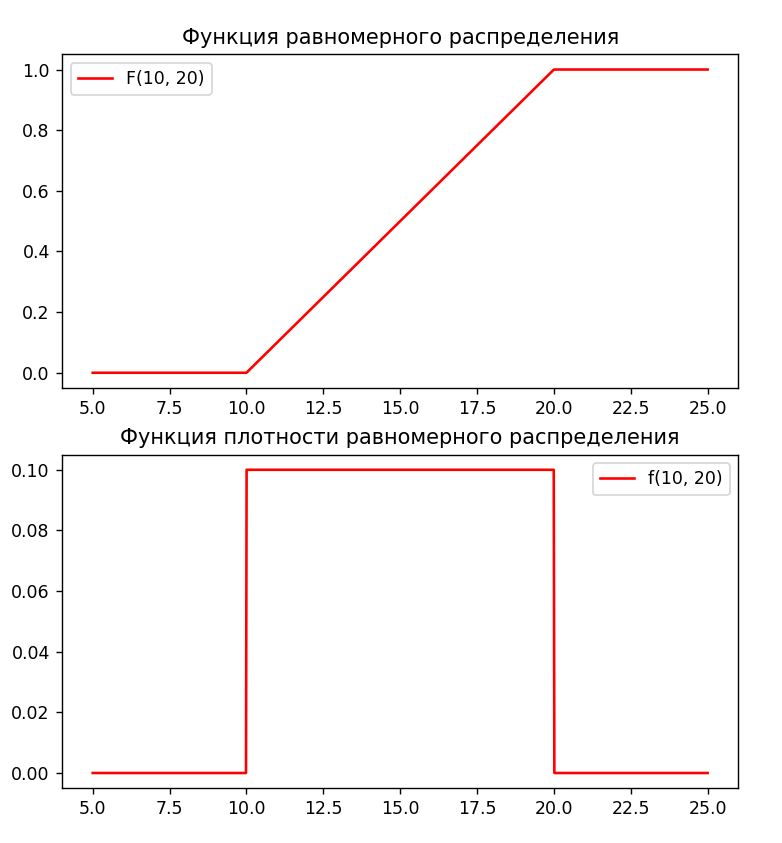
\includegraphics[scale = 1]{1.jpg}
	\label{fig:screenshot001}
	\caption{при a = 10, b = 20}
\end{figure}

\begin{figure}[h]
	\centering
	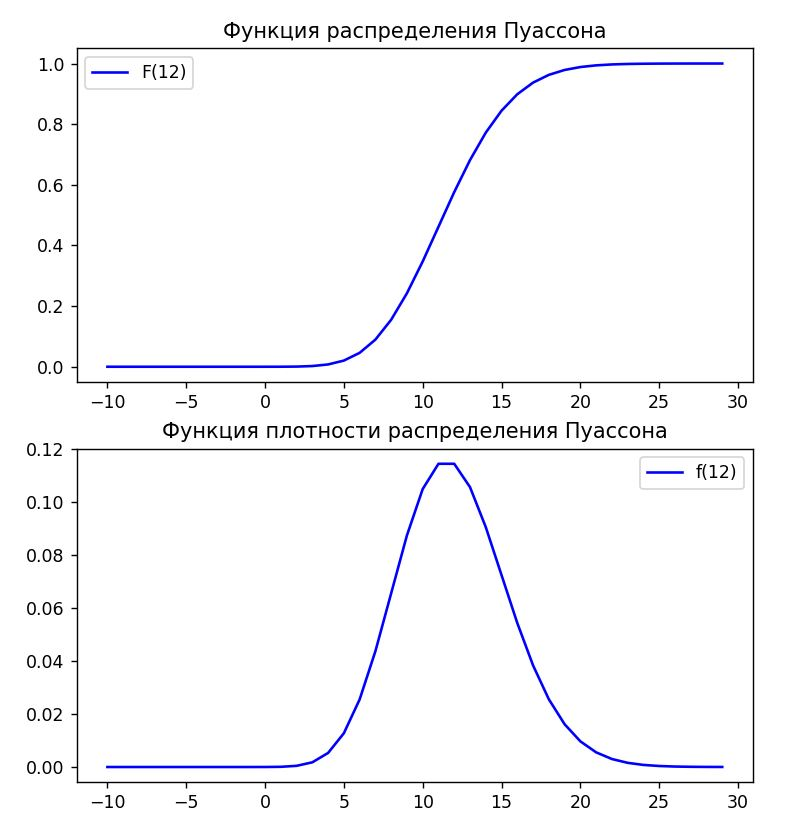
\includegraphics[scale = 1]{2.jpg}
	\label{fig:screenshot002}
	\caption{при $\lambda$ = 12}
\end{figure}

\begin{figure}[h]
	\centering
	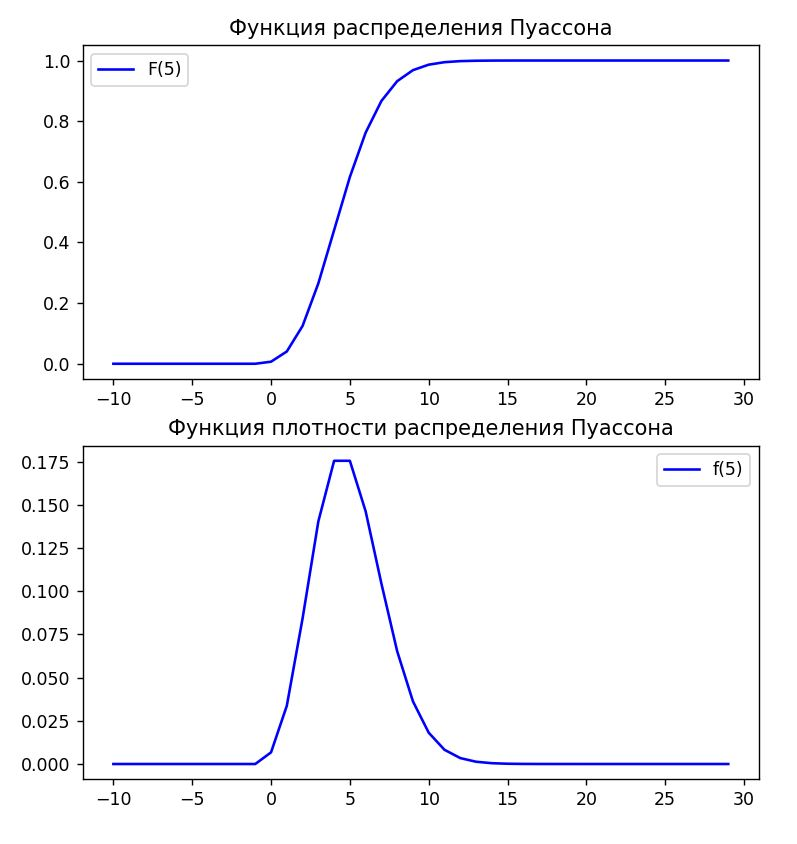
\includegraphics[scale = 1]{3.jpg}
	\label{fig:screenshot003}
    \caption{при $\lambda$ = 5}
\end{figure}
\end{document}
